% Created 2023-02-01 Wed 20:57
% Intended LaTeX compiler: pdflatex
\documentclass[11pt]{article}
\usepackage[utf8]{inputenc}
\usepackage[T1]{fontenc}
\usepackage{graphicx}
\usepackage{longtable}
\usepackage{wrapfig}
\usepackage{rotating}
\usepackage[normalem]{ulem}
\usepackage{amsmath}
\usepackage{amssymb}
\usepackage{capt-of}
\usepackage{hyperref}
\hypersetup{colorlinks=true,linkcolor=blue}
\author{Aditya Yadav}
\date{\today}
\title{Revision}
\hypersetup{
 pdfauthor={Aditya Yadav},
 pdftitle={Revision},
 pdfkeywords={},
 pdfsubject={Basic revision from the classes from previous sem},
 pdfcreator={Emacs 30.0.50 (Org mode 9.6.1)}, 
 pdflang={English}}
\begin{document}

\maketitle
\tableofcontents


\section{Grammer Type ( Noam Chomsky Classification )}
\label{sec:org13d349d}
\begin{center}
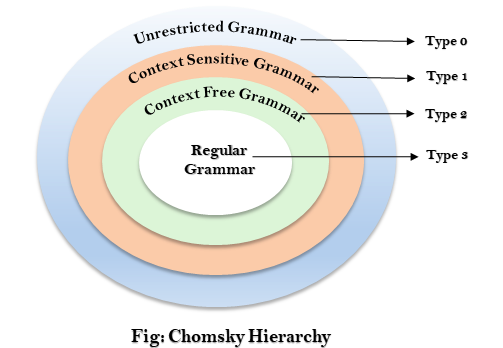
\includegraphics[width=.9\linewidth]{Revision/type_grammer.png}
\end{center}
\subsection{Type 0 ( unrestricted Grammer )}
\label{sec:orgec06a67}
\begin{enumerate}
\item \(\alpha\) -> \(\beta\)
\item \(\alpha\) \(\in\) (V+T)\textsuperscript{+}
\item \(\beta\) \(\in\) (V+T)\textsuperscript{+}
\end{enumerate}
Example -> AB -> \(\epsilon\)
Not a Example -> \(\epsilon\) -> A
\subsection{Type 1 ( Context Sensitive Grammer ) ( CSL )}
\label{sec:orgb3c5111}
\begin{enumerate}
\item Must be a Type-0
\item |\(\alpha\)|  \(\le\) |\(\beta\)|
\end{enumerate}
Not Example -> AB -> \(\alpha\)
\subsection{Type 2 ( Context Free Grammer ) ( CSL )}
\label{sec:org40aab5b}
\begin{enumerate}
\item Must be Type-1
\item V -> (V+T)\textsuperscript{+}
\end{enumerate}
\subsection{Type 3 ( Regular Grammer )( RG )}
\label{sec:orge6d5e0f}
\begin{enumerate}
\item Must be Type-2
\item V => T\textsuperscript{*}  \texttimes{} V / T\textsuperscript{*} -> Right linear Grammer
OR
V => V \texttimes{} T\textsuperscript{*} / T\textsuperscript{*} -> Left linear Grammer
\end{enumerate}
\section{Ambigious grammer}
\label{sec:org1e94aee}
\subsection{Defination}
\label{sec:org1ca8d95}
Ambigious grammer -> A grammer which can derive multiple parse trees for an input string it is called a ambigious grammer.
\subsection{Conversion from ambigious to unambigious grammer}
\label{sec:org6b7c8aa}
\begin{itemize}
\item Converting a ambigious grammer to unambigious grammer is not always possible.
\item There is no algorithm for converting unambigious grammer to ambigious grammer.
\item Ambigious grammers from which ambigity can't be remvoed are known as inherently ambigious grammer.
\item A language is said to be ambigious if all the grammers that generate that language are ambigious.
\end{itemize}
\subsubsection{By Asssigning priority}
\label{sec:orgce4ba3f}
S -> id/S+S/SxS -> Removal Ambiguity
Priority S -> S+T/T
         T -> TxF/F
         F -> id
The bottom productions has the highest priority and the higher we go the less priority that productions get.
\subsubsection{Left factoring}
\label{sec:org1e05d5e}
in the below case the first grammer will cause the compiler to be confused as if a string starting with 'a' comes it will not be sure which of the productions to use.
Ex-> W = ad
S -> ab/ac/ad
to
S -> aS'
S' -> b/c/d
\begin{enumerate}
\item Example
\label{sec:orge707cdd}
S -> a/b/c/iEtS/iEtSeS
to
S -> a/b/c/iEtsP/iEtsSP
P -> eS/\(\epsilon\)
\end{enumerate}
\subsubsection{Recursion}
\label{sec:org41fa57f}
\begin{enumerate}
\item Types recursion
\label{sec:org764c127}
If the grammer contains left recursion then top down parser will go to infinite loop.
\begin{center}
\begin{tabular}{ll}
\hline
Left Recursion & Right Recursion\\[0pt]
\hline
S -> Sa/b & S -> aS/b\\[0pt]
\hline
\end{tabular}
\end{center}
\item Conversion
\label{sec:orgcce62db}
A -> Aa/B  ------- It has a recusion part Aa and a non recursion part and we try to seperate them
to
A -> BA'
A' -> aA'/\(\epsilon\)
\item Example
\label{sec:orgd814801}
E -> E+T/T
T -> T*F/F
F -> id/(E)
to
E -> TE'
E' -> +TE'\emph{\(\epsilon\)
T -> FT'
T' -> *FT'}\(\epsilon\)
F -> id/(E)
\end{enumerate}
\section{Compiler}
\label{sec:org582118f}
\begin{enumerate}
\item Processor can directly take high level language program also but it will take a lot of time, hence to make it faster we use a compiler as the processor will compile or covert the program each time it runs the program but the compiler only converts it only once.
\item Compilation in java in compiler is faster than c-compiler as it does coversion up to the intermediate code generation stage only hence each time the program runs these last two stages are executed making to slower than c execution.
\end{enumerate}
\begin{center}
\begin{tabular}{lllllllllll}
\hline
Language Processing & --HLL--> & Pre Processor & ---Pure HHL---> & Compiler & -----Multi Assembly Language----> & Assebler & ---Multi Relocatable code----> & Linker & -------Single Relocatable Code-> & Loader\\[0pt]
 &  &  &  &  &  &  &  & Cousins of Compiler &  & Ready State\\[0pt]
\hline
\end{tabular}
\end{center}
\subsection{Lexical Analyzer}
\label{sec:org3a178ed}
\begin{enumerate}
\item Lexical analyzer will generate a token only when parser asks for it.
\item First phase of the compiler is called lexical analyzer. It is also called scanner.It will divide the given program into meaningful strings know as token.
\end{enumerate}
\subsubsection{Functions}
\label{sec:orgc68ab65}
\begin{enumerate}
\item Dividing the program into tokens
\item It will eliminate the comment lines
\item It will eliminate the whitespace chracters(tab,$\backslash$, ,"\n").
\item It will help in giving error message by providing the line number.
\end{enumerate}
\subsection{Parser}
\label{sec:org37ef6c7}
The process of deriving string from a given grammer is called derivation or parsing
\subsubsection{Types of parser}
\label{sec:org546af25}
\begin{enumerate}
\item Top down Parser
\label{sec:org5002176}
These are also called LL(Left to Right,Left most derivation) parsers.
It start with root or starting symbol and proceeds to children that is String.
\begin{enumerate}
\item Top down parsers use leftmost derivation.
\item All the parsers perform left most derivation only and none of them gives right of most derivation.
\item Difficulty with top down parsers is that when a variable has more than 1 choice it has to choose the correct production by backtracing.
\end{enumerate}
\begin{enumerate}
\item Recursive descent Parser (LL(0))
\label{sec:org00da211}
\begin{enumerate}
\item In Recursion descent Parser we use leftmost Derivation.
\item In Recursion descent Parser we will write one function for every variable
\item If the grammer contains left Recursion the parser will go into infinite loop.
\item If the grammer contains sometimes we will get parsing error.
\item Lot of time is wasted in back tracing so time complexity of Recursion descent Parser is O(2\textsuperscript{n}).
\end{enumerate}
\begin{verbatim}
S(){
    choose any production S -> x1,x2,x3,x4.....xk of S
    for(i=1 to k){
       if (xi is variable) { x1() ;}
       else if (xi == look ahead symbol) { then increment input pointer;}
       else { Error {back track} }
    }
}
\end{verbatim}
\item Predective Parser (LL(1))
\label{sec:orgc2d68a8}
\end{enumerate}
\item Bottom Up parser
\label{sec:org758c573}
\begin{enumerate}
\item It start from the children or the string and proceeds to root or the starting symbol.
\item It uses reverse of right most derivation.
\item The Different with bottom up parser is identifying a substring or handle which will give a required variable to get to the start symbol.
\end{enumerate}
\end{enumerate}
\section{Question}
\label{sec:org6567898}
\subsection{Q1}
\label{sec:orga72f52d}
Write a CFG for Language L = \{ a\textsuperscript{m} | m \(\ge\) 1 \}
Ans. S -> aS | a
\subsection{Q2}
\label{sec:org42a03fd}
Write a CFG for Language L = \{ a\textsuperscript{m} b\textsuperscript{n} | m,n \(\ge\) 1\}
Ans. S-> AB 
     A-> Aa | a 
     B-> Bb | b
\subsection{Q3}
\label{sec:org6e48c41}
How many possible DFA's are there with 2 states X and Y, where X is an initial state over alphabet \{a,b\}?
\begin{center}
\begin{tabular}{lll}
\hline
N/NF & X & Y\\[0pt]
\hline
X & a/b & a/b\\[0pt]
Y & a/b & a/b\\[0pt]
\hline
\end{tabular}
\end{center}
Here we can set either X or Y or neither or both as final states so we have to multiple the table result with 4
ans = 4 * 4 * 4 = 64
\subsection{Q4}
\label{sec:org5014881}
\emph{\emph{\emph{\emph{TO Complete/}}}}
Draw the parse tree of this statement?
S -> aS/Sa/a
W -> aaa

\begin{center}
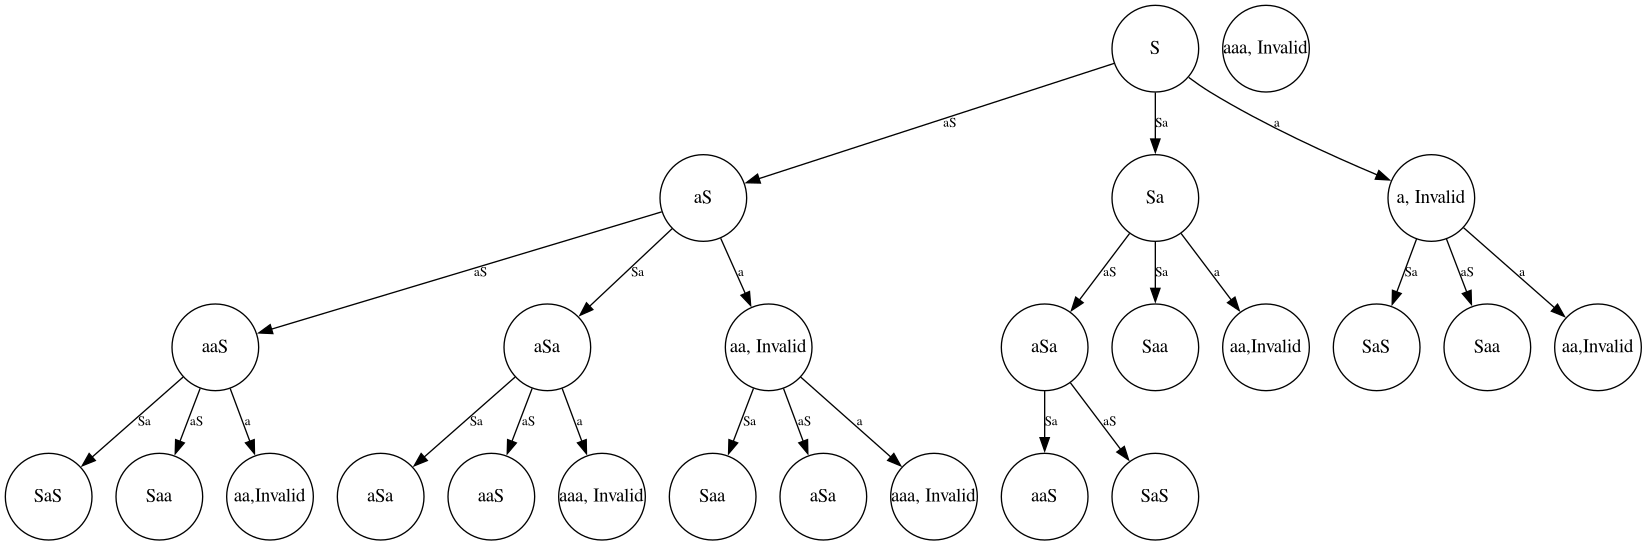
\includegraphics[width=.9\linewidth]{Revision/Q4.png}
\end{center}
\end{document}